This chapter investigates \ref{rq:3} by exploring the challenges in the operational management of \acp{DTE} that involve the management of multiple \acp{DT} from a deployment and runtime perspective.
%
Several \acp{DT} need to be orchestrated on a cyber-physical computing infrastructure, ensuring that \acp{DT} are able to interact with the \acp{PA} they represent and maintain the target level of performance and synchronization. 
%
This problem is further exacerbated when considering that \ac{DTE} can involve \acp{DT} developed for different platforms, and computing infrastructures that span the whole \emph{edge-cloud continuum}. 

Motivated by these challenges, this chapter introduces the concept of a \emph{\ac{DTC}}, a middleware that aims to facilitate the operational management of \acp{DTE} by providing a unified interface to manage the deployment and runtime of \acp{DT} across heterogeneous \ac{DT} platforms and computing infrastructures.
%
This proposal complements the \ac{HWoDT} approach presented in Chapter~\ref{chap:dte:hwodt}, which focuses on the interaction with \ac{DTE}, rather than their operational management. 

The chapter analyzes the challenges in the operational management of \acp{DTE}, and presents a proposal for an architecture of the \ac{DTC} middleware. The functionalities are supported by a set of \emph{descriptions} that can inform the \ac{DTC} about the characteristics of the \acp{DT} and \acp{PA} involved in the \ac{DTE} and support stakeholders in having a clear understanding of the system state at any stage.


%=======================================================
\section{Operational Challenges}
%=======================================================

An orthogonal aspect of complexity when developing a \ac{DT} is understanding its non-functional requirements that allow for considering the \ac{DT} effectively synchronized.
%
The concept of \emph{entanglement}~\cite{dt-IoT-context-Minerva-2020} has been used to define the level of synchronization of the \ac{DT} with the \ac{PA} and can be measured with metrics that include network latency and computation time on both the physical device and the computing node that is running the \ac{DT}~\cite{bellavista2024odte}.

In recent years, with the increased availability of computing resources at the edge of the network, the concept of edge-cloud continuum has emerged as a paradigm to distribute computation across a variety of computing nodes, obtaining benefits in terms of latency and optimizing the overall workload of an \ac{IoT} system~\cite{Rosendo_Costan_Valduriez_Antoniu_2022}.
%
Like other \ac{IoT} system components, \acp{DT} can also be deployed within the continuum~\cite{Bellavista_Bicocchi_Fogli_Giannelli_Mamei_Picone_2024} with trade-offs in terms of entanglement, cost and resource availability.
%
The advantages of this approach, though, are offset by additional complexity in the operational management of the software system.
When it comes to \acp{DT}, this means choosing the suitable computing node to deploy the \ac{DT} software, to ensure the \ac{QoS} requirements are matched at runtime.
This can be challenging due to the cyber-physical nature of \acp{DT}.
Additionally, when several \acp{DT} are employed as parts of an ecosystem sharing the same computing infrastructure, it should be possible for operators to easily navigate the continuum and observe performance metrics to understand the potential impact of deploying new \acp{DT} in the system and eventually reconfigure it to balance the overall workload.

On the development side, the heterogeneity of \ac{DT} platforms poses additional challenges as they may constrain the ability to deploy a \ac{DT} across the edge-cloud continuum.
%
Indeed, while open-source platforms can be adapted to run on a generic infrastructure, proprietary ones are usually Platform as a Service solutions, bound to the cloud infrastructure. 
%
Developers tasked with implementing a \ac{DT} must hence evaluate the suitability of a given \ac{DT} platform, taking into consideration both the functional (i.e., meta-model, features, services) and non-functional (i.e., latency, computing power, privacy) requirements.

Since these requirements may vary significantly depending on the \ac{PA} being modeled it is realistic to assume that a complex \ac{DT}-based system may include \acp{DT} developed on different platforms.
%
This has surfaced challenges in the management of the development and deployment of \ac{DT}-based systems which may need to guarantee the \ac{QoS} requirements of \acp{DT} developed with heterogeneous technologies and platforms while managing a shared pool of heterogeneous computing resources.

The proposal of the \ac{DTC} aims to address the following goals:
\begin{itemize}
    \item \textbf{reducing deployment complexity} of a \ac{DT}-based system integrating \acp{DT} developed for different platforms sharing the same computing infrastructure.
    \item \textbf{facilitating the interaction of different stakeholders} with a \ac{DT}-based system enabling easy access of relevant information over the development-to-deployment lifecycle of \acp{DT}.
\end{itemize}

%========================================================
\section{Phases and Stakeholders}
%========================================================


The process of developing and managing a \ac{DTE} involves several critical phases, each essential for the effective development, discovery, selection, deployment, and operation of \acp{DT}.
%
These phases abstract the development-to-deployment lifecycle of \acp{DT} in a structured approach which is independent of the target application domain or specific technological choices.

Identifying these phases helps shape the requirements for the \ac{DTC} and understand the roles of the stakeholders that are involved in each phase.


\paragraph{DT Software Capabilities Discovery \& Selection}
As a starting point, every DT system is originating from the needs of a cyber-physical context.
%
This usually involves one or several \emph{\ac{PA} Owner} who are the stakeholders that possess the knowledge about the \acp{PA} and the goal that requires \acp{PA} to be modeled and digitalized~\cite{michael2024software}.
The \emph{\ac{PA} Owner} is also in charge of granting access to the \ac{PA} data and sensors. 
%
The first phase hence focuses on identifying DT capabilities that align with specific application and use case requirements.
%
This phase involves defining the functionalities of the DT, associating it with the corresponding physical asset category, specifying communication protocols, and detailing its properties, events, relationships, and available actions. 
%
Notably, an asset might have multiple owners.
For instance, an industrial machine is produced by a manufacturer and acquired by a company to employ it in one of its facilities.
The same machine is then owned simultaneously by the manufacturer who may have control of telemetry data and be interested in monitoring the machine to offer predictive maintenance services, by the company who might want to keep track of all the machines across facilities and by the facility manager who might monitor the state of operational of the machine in the specific production line it is employed. 
All the owners may have access to different data and model the same asset with different target goals.


\paragraph{DT Development and Platform Selection}

A \emph{\ac{PA} Owner} may commission the development of a \emph{DT Developer} to implement the DT for the PA. The developer will implement a DT using a target technological stack, that depends on their expertise and the availability of the computing infrastructure that is available for the deployment of the DT.
%
In this phase it is necessary to ensure that the chosen DT requirements can be effectively implemented on a specific platform.
%
This phase involves defining platform-specific configurations, including implementation details, required configuration parameters, and technical requirements.
%
Notably, the \emph{\ac{PA} Owner} is usually the (virtual) owner of the computing infrastructure on which the DT will be eventually deployed. When the DT is developed as commissioned by the \emph{\ac{PA} Owner} this may influence the technological choices of the \emph{\ac{DT} Developer}.
%
This doesn't always need to be the case though, it can be reasonably expected that in the near future \acp{DT} implementations for specific kinds of assets would be made available to owners of such assets either publicly or commercially.
These would be implemented either by manufacturers or a community of \emph{\ac{DT} Developers}.
Such reusable \acp{DT} would then be implemented with a given technological stack and need to be deployed on the available resources of the \emph{\ac{PA} Owners}, in order to be configured and connected to the locally available \acp{PA}. 
Similarly, such reusable \acp{DT} could be offered as-a-service and made available only as instances deployed on commercial platforms. This adds a further layer of complexity to the management of the computing infrastructure running the possibly different \acp{DT} in an organization.


\paragraph{Digital Twin Deployment}

Once a DT is developed (from scratch or reusing existing implementations) the next goal is to run it on a computing infrastructure.
This step involves a \emph{DT Operator} who have knowledge about the \ac{DT} requirements and can configure the computing infrastructure to make sure that the DT is deployed correctly and gets access to the \ac{PA} data streams (this can be the same person as the \emph{DT Developer} in a typical Dev-Ops fashion).
%
Deploying a DT can be a challenging task, involving several steps that depend on the complexity of the deployment infrastructure and the requirements of the DT.
%
This phase is crucial to ensuring that all deployment conditions are met, including 
the availability of deployable artifacts, and the correct setup of communication configurations, enabling interaction with both physical and digital entities.
%
In a computing continuum, a DT may need to be deployed at different levels either on the edge, fog or cloud depending on the admissible trade-offs between network latency and computing power requirements. Notably, \acp{DT} might need to be moved across this continuum for a variety of reasons, either being connectivity requirements with the \ac{PA} (and thus a DT may move horizontally in the continuum) or changes in synchronization requirements or scaling (and thus moving vertically in the continuum). Finally, the same \ac{PA} could be connected to different \acp{DT} replicas, serving different use cases~\cite{dt-IoT-context-Minerva-2020}.

\paragraph{Running Digital Twin}

The last phase starts once the \ac{DT} is up and running. In this phase the DT must be identified, described, and reachable by consumers.
%
This phase is critical for maintaining an accurate and up-to-date representation of the DT instance, managing its interaction protocols, handling lifecycle transitions, and enabling real-time state monitoring and interaction with the twin.
%
The ability to monitor information about running \acp{DT} is essential for ensuring synchronization with physical assets, supporting advanced digitalization processes, and facilitating interoperability within complex cyber-physical systems.


\begin{figure}
    \centering
    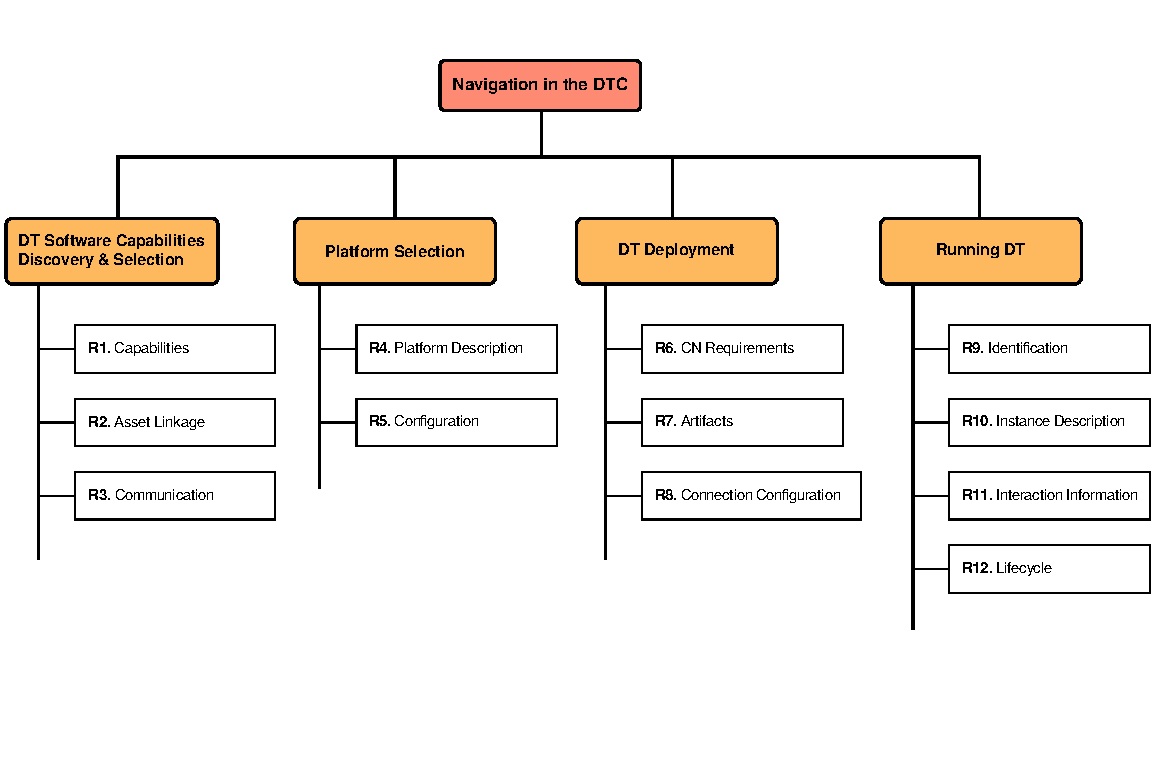
\includegraphics[width=0.9\textwidth]{figures/dtc/dtc-requirements.pdf}
    \caption{Phases and requirements for managing \acp{DT} in a \ac{DTC}.}
    \label{fig:dtc-requirements}
\end{figure}

\Cref{fig:dtc-requirements} summarizes the \emph{information} requirements for managing \acp{DT} across these phases, namely what kind of information is necessary to support stakeholders in each phase, and ensure that the phase can run successfully.
%
These requirements guide the design of \emph{descriptions} that can be used to inform the \ac{DTC} about the characteristics of the \acp{DT} to deploy and manage, in a platform-agnostic way.


%=======================================================
\section{Key Elements and Descriptions}
%=======================================================

To address the challenges in the operational management of \acp{DTE}, the \ac{DTC} relies on a set of key elements and their structured descriptions that provide a structured way to represent and manage the various components involved in a \ac{DTE}.

\begin{table}
    \centering
    \small
    \begin{tabular}{p{2cm} p{8.5cm} p{2cm}}
    \toprule
    \textbf{Entity} & \textbf{Description} & \textbf{Req.} \\
    \hline
    \textbf{Physical Asset Schema (PAS)} & Defines the abstract capabilities and interaction patterns of a specific type of industrial asset (e.g., robotic arm, conveyor system). Provides essential metadata for communication protocols, API definitions, and interface configurations without specifying instance-specific values like IP addresses or credentials. & R1, R2, R3 \\ \hline
    \textbf{Physical Asset Instance (PAI)} & Represents a deployed instance of an asset as defined by the PAS. Includes instance-specific configurations like network settings, authentication credentials, and protocol-specific settings. Facilitates the runtime communication between the DT and the physical asset. & R1, R2, R3 \\ \hline
    \textbf{Digital Twin Schema (DTS)} & Defines the capabilities, behaviors, and structural components of a Digital Twin, linking the digital representation to its corresponding physical asset. Specifies properties, events, relationships, actions, and fidelity between the physical and digital counterpart. & R1, R2, R3 \\ \hline
    \textbf{Digital Twin Package (DTP)} & Defines the platform-specific implementation of the DTS, including code, configuration parameters, and dependencies required for deployment. Ensures the fidelity and communication requirements of the DTS are met during deployment. & R6, R7, R8 \\ \hline
    \textbf{Digital Twin \-  Instance (DTI)} & Represents a running instance of the Digital Twin, including metadata for orchestration, monitoring, and lifecycle management. Tracks software lifecycle states and exposes relevant runtime metrics. Ensures the connection between the DTC and the deployed DT instance. & R9, R10, R11, R12 \\
    \hline
    \textbf{Runtime Platform (RP)} & Describes the underlying computing infrastructure and environment where the Digital Twin is deployed. This includes details about the hardware, software, and network configurations that support the DT's operation. & R4, R5 \\
    \bottomrule
    \end{tabular}
    \caption{Overview of DTC Entities: Characteristics, Responsibilities, and Associated Requirements}
    \label{table:dtc_descriptions_requirements}
\end{table}


At the core of this descriptive framework is the \textit{Physical Asset Schema} (PAS), which serves to uniquely define a specific \textit{type} of industrial asset---such as a robotic arm, conveyor system, or CNC machine.
%
The PAS encapsulates essential metadata that describes how assets of this category are expected to interact within a digital environment. This includes supported communication protocols (e.g., MQTT, OPC UA, HTTP), standardized API definitions, and more broadly, the configuration of interfaces and interaction models required for monitoring, control, and integration across systems. It is important to note that the PAS does not contain instance-specific values such as IP addresses, port numbers, or credentials. Instead, it provides a structured description of the expected capabilities and modes of interaction for devices of a given type.
%
This is similar to the concept of \emph{Thing Model} in the context of the \ac{WoT}~\cite{wot-td} which only focuses on capabilities and abstracts completely from protocols and implementation details. The PAS, instead, includes this information, as it is more closely related to the physical devices and not on their virtual \emph{Thing} representation. 

This schema is essential for the \ac{DTC} to understand how different \ac{PA} conform to specific interaction patterns and how to configure communication with them. 

Building upon the PAS, the \textit{Physical Asset Instance} (PAI) represents a deployed instance of an asset as defined by the PAS.
%
While the PAS defines the abstract capabilities and expected interaction patterns of a category of assets, the PAI provides the concrete, instance-specific configuration required for operational integration. This includes network information (such as IP addresses and ports), authentication credentials, and protocol-specific settings like MQTT topics or OPC UA node identifiers.
%
These configurations are essential to enable runtime communication between the DT and the physical asset, supporting dynamic discovery, secure interfacing. As such, the PAI forms the operational bridge that links the abstract asset description to real-world deployment contexts, ensuring that the DT can monitor and interact with its physical counterpart in a precise and reliable manner.
%
The \ac{WoT} \ac{TD} can be used for this scope as it includes the necessary information to describe how to connect to a specific device instance.

Following the same principles and responsibilities of the PAS, the \textit{Digital Twin Schema} (DTS) defines the capabilities and behaviors of a DT independently of any concrete implementation.
%
It establishes a reference to the corresponding \ac{PA} category, ensuring semantic linkage between the physical and digital representations. The schema outlines the structural components of the DT, such as its properties, observable events, defined relationships, and available actions. It also specifies the target \emph{fidelity} of the DT, capturing the mirrored functionalities of the physical counterpart within a given context and under specific application goals.

The \textit{Digital Twin Package} (DTP) represents instead the software implementation of a given schema on a target \ac{DT} platform.
%
The package includes all platform-specific implementation artifacts required for deployment and execution.
%
It incorporates the executable code, configuration parameters, and platform dependencies, ensuring compliance with the DTS's fidelity and communication requirements.
%
It also provides detailed bindings for the declared communication protocols---e.g., how MQTT is used to interface with physical assets and how HTTP APIs enable interaction with external digital services.

When a package is deployed within the DTC, it gives rise to a \textit{Digital Twin Instance} (DTI).
%
This instance represents the active, running version of the DT within the operational infrastructure and includes all metadata necessary for orchestration, monitoring, and software lifecycle management.
The DTI maintains references to its originating schema and the platform on which it is deployed, along with essential access information such as IP addresses, ports, and authentication tokens. It also exposes relevant runtime metrics—including CPU, memory, and network utilization—as well as any endpoints required to access its services and functionalities.
%
In addition, the DTI tracks and exposes the \ac{DT} connectivity information tracking whether the \ac{DT} is connected to the \ac{PA}. These lifecycle states pertain strictly to the operational status of the deployed software component and are independent of the internal logic or functional behavior of the DT itself (differently from the synchronization lifecycle discussed in \Cref{sec:dte:engineering-dt:dt-lifecycle}).
%
Functional state and domain-specific behavior remain under the responsibility of the DT and are communicated through its defined interfaces in the digital space (e.g., through the \ac{DTKG} if considering a \ac{HWoDT} ecosystem \Cref{chap:dte:hwodt})

With reference to the requirements identified in \Cref{fig:dtc-requirements}, \Cref{table:dtc_descriptions_requirements} summarizes the key elements and their associated responsibilities in supporting the operational management of \acp{DTE}.
%
The integration of the PAS, PAI, and DTS effectively addresses the core requirements \textbf{R1.Capabilities}, \textbf{R2.Asset Linkage}, and \textbf{R3.Communication}, which are focused on the representation of features of the \acp{PA} and \acp{DT}, the relationship that links a \ac{DT} to a specific \ac{PA}, and the necessary communication protocols.
%
These descriptions support the \emph{DT Software Capabilities Discovery \& Selection} phase, enabling stakeholders to explore available \acp{PA} and their corresponding DT types based on defined capabilities and interaction patterns.
%
Additionally, the DTP supports requirements \textbf{R6.Computing Node Requirements}, \textbf{R7.Artifacts}, and \textbf{R8.Connection Configuration}, which pertain to platform-specific aspects to support the creation of DT instances within the DTC and can hence support the \emph{Digital Twin Deployment} phase.

The DTI is responsible for addressing the requirements \textbf{R9.Identification}, \textbf{R10.Instance\- Description}, \textbf{R11.Interaction\- Information}, and \textbf{R12.Life\-cycle}, which in the \emph{Running Digital Twin} phase support stakeholders in the identification of the DT instance, the discovery of its status and interaction descriptions, as well as its connectivity with the \ac{PA} during operation.


\textbf{R4.Platform Description} and \textbf{R5.Configuration} are supported by the \textit{Runtime Platform} (RP) description.
%
Differently from the other descriptions, these are tied to the computing infrastructure and the target platforms on which the \ac{DT} can be deployed. 
%
\textbf{R4}, includes platform-dependent attributes such as the platform type, supported communication protocols, and data formats, enabling the DTC to match DTPs to the correct platform.
%
Additionally, \textbf{R5} plays a crucial role in establishing the necessary parameters and operational requirements specific to the platform and implementation. Proper configuration ensures that the DT functions optimally by aligning its settings with platform constraints, communication protocols, and performance expectations.  

Together, these components support stakeholders to seamlessly identify and discover managed \acp{PA}, understand their capabilities, and determine the availability of corresponding \ac{DT} packages for deployment. This structured approach ensures that the DTC facilitates efficient asset discovery, aligns with system interoperability needs, and supports dynamic integration across diverse environments. 

%=======================================================
\section{Architecture of the \acl{DTC}}
%=======================================================

\begin{figure}
    \centering
    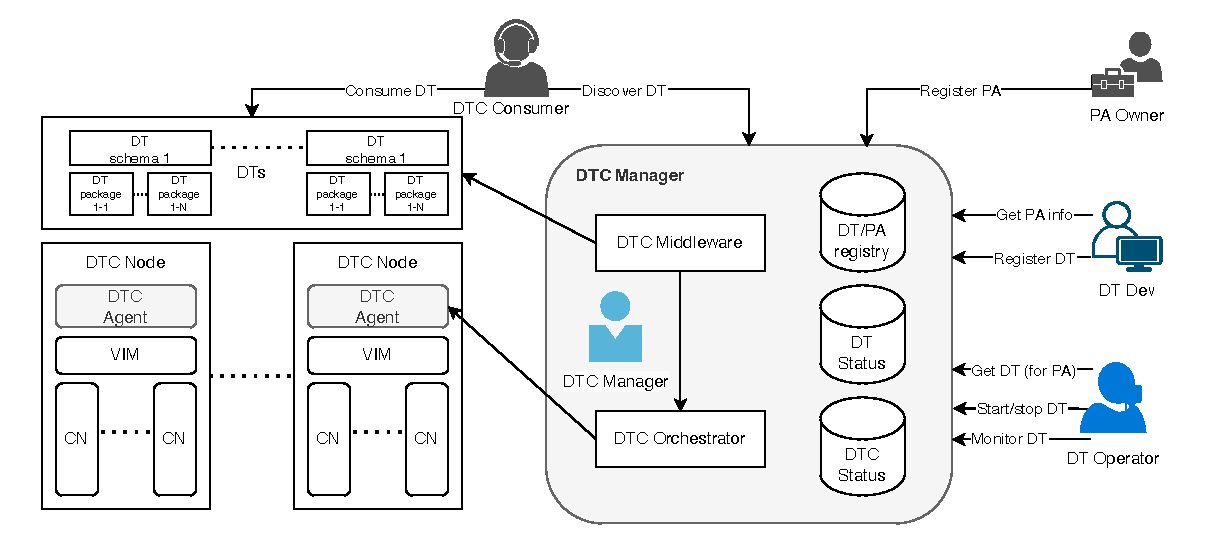
\includegraphics[width=\textwidth]{figures/dtc/architecture_new_v2.pdf}
    \caption{Functional Architecture of the \ac{DTC} with the main components and the interactions with stakeholders.}
    \label{fig:dtc-architecture}
\end{figure}

The aim of the DTC is to create a new open-system perspective of connected, interoperable and pervasive DTs modeled and engineered to create an effective cyber-physical abstraction layer.
%
This requires, first, facilitating the execution of DTs on a set of DT platforms.
Second, by exploiting the advantages of a broad compute continuum of cloud and edge resources, to deploy the DTs on the \textit{best} Compute Node (CN) available to guarantee application requirements.
%
The architecture of the DTC is depicted in \Cref{fig:dtc-architecture} and includes DTC functional blocks (grayed boxes), infrastructure modules, DT artifacts, while highlighting the interactions of DTC stakeholders. 

Other than the already introduced roles of \emph{PA Owner}, \emph{DT Developer}, and \emph{DT Operator}, we introduce the roles of \emph{DTC Manager} and \emph{DTC Consumer}.
%
The \emph{DTC Manager} is in charge of managing an instance of the middleware that servers the functionalities of the DTC across the available computing nodes in the target infrastructure.
%
The \emph{DTC Consumer} is anyone (with access to the DTC) interested in exploiting the functionalities of one or more \acp{DT} deployed on the DTC.
%
The DTC serves such users in discovering which \acp{DT} are available, what features such \acp{DT} offer and enabling to connect with \acp{DT} once found in order to exploit their APIs and services. DTC Consumers are hence DT Consumers, which make use of the DTC abstraction to connect with the \acp{DT} of interest, to possibly develop applications on top of the services offered by such \acp{DT}. 

%----------------------------------------
\subsection{Functional Overview}
%----------------------------------------

From a high-level perspective, the DTC allows DT operator to expose a collection of DTs for use of DT Consumers.
%
Each DT is described by a \emph{schema}, which in turn is associated with a certain number of DT \emph{packages}, allowing their deployment on different platforms.
%
New DT schemas and DT packages can be dynamically onboarded on the DTC by DT Developers.

DT packages are used to create and execute DT instances on the DT platforms, each running on a CN. A CN in turn can be implemented as a virtualized environment or as a bare infrastructure covering the full compute continuum. 

To mask all the deployment complexity, an intermediate DTC Manager is introduced, which will be responsible for interacting with all DTC stakeholders.
\acp{DT} can be deployed across the compute continuum on top of DTC nodes.
%
Each DTC node is a collection of computing nodes orchestrated by a Virtual Infrastructure Manager (VIM). A typical practical example of such collection of CNs is a Kubernetes cluster, orchestrated by a cloud-control manager.
%
While the VIM handles low-level resource management of computing resources, a DTC Agent is responsible for managing and monitoring the execution of \acp{DT} within the DTC node. Each DTC Agent will be in turn controlled by the DTC manager, orchestrating and coordinating the execution of \acp{DT} across the continuum.

More in detail, a DT Operator willing to create a new DT corresponding to a given schema, contacts the DTC Manager, who will be responsible for:
\begin{inlinelist}
    \item identifying the platforms and the corresponding DT packages based on the DT schema and the DT's fidelity requirements;
    \item configuring the communication and computing resources accordingly.
\end{inlinelist}

Rather than being acted by a human, the DTC Manager role can be implemented by two software components:
\begin{itemize}
    \item \textbf{DTC Middleware} is the front-end for any requests from the various stakeholders and is responsible for managing the DT/\ac{PA} registry, storing all the descriptions introduced in \Cref{table:dtc_descriptions_requirements}, and exposing the necessary APIs to interact with the DTC;
    \item \textbf{DTC Orchestrator} is responsible for instantiating \acp{DT} by configuring the underlying resources to enable the proper functioning of the \acp{DT}. This process is performed by the DTC Orchestrator through the various DTC agents, which in turn have control of DTC nodes through their respective VIMs. The separation of DTC Agents and VIMs allows the DTC orchestrator to seamelessly interact with DTC nodes, regardless of their underlying virtualization infrastructure.
\end{itemize}

A \ac{PA} Owner willing to associate a \ac{PA} to the DTC will issue a PA-registration request to the DTC orchestrator, which will record the existence of the \ac{PA} within the DT/\ac{PA} registry storing the PAS and PAI descriptions.
%
Moreover, it will ensure the \ac{PA} can be reached by the DTC nodes by configuring the underlying networking infrastructure, e.g., configuring IoT device, network appliances or virtualized components, to build and setup all the prerequisites required to run target \acp{DT} on the reference platforms (e.g., add a record on a routing table or update a firewall entry to enable the correct communication). 


A DT developer will be able to obtain information regarding existing \acp{PA}, in order to develop DTs that can interact with them.
%
When deployment is complete a DT developer will be able to register a DT within the platform by contacting the DTC middleware. This operation will add the DT to the DT/\ac{PA} registry, enabling their execution when needed by providing the DTS and DTP.

When the \ac{DT} is required to be deployed, a DT operator will be able to manage the execution of \acp{DT} through the DTC Manager.
Through the DTC Middleware the operator will be able to: \begin{inlinelist}
    \item retrieve a DT for a specific PA,
    \item start/stop a DT,
    \item monitor the execution status of a DT
\end{inlinelist}.

Finally, a DTC Consumer willing to access a DT within the DTC, contacts the DTC Middleware, who will be responsible for looking up for a DT having the required characteristics and providing the necessary hooks for the consumer. The DTC consumer will be then able to interact directly with the DT through its API.


%----------------------------------------
\subsection{Interaction Example}
%----------------------------------------


\begin{figure}
    \centering
    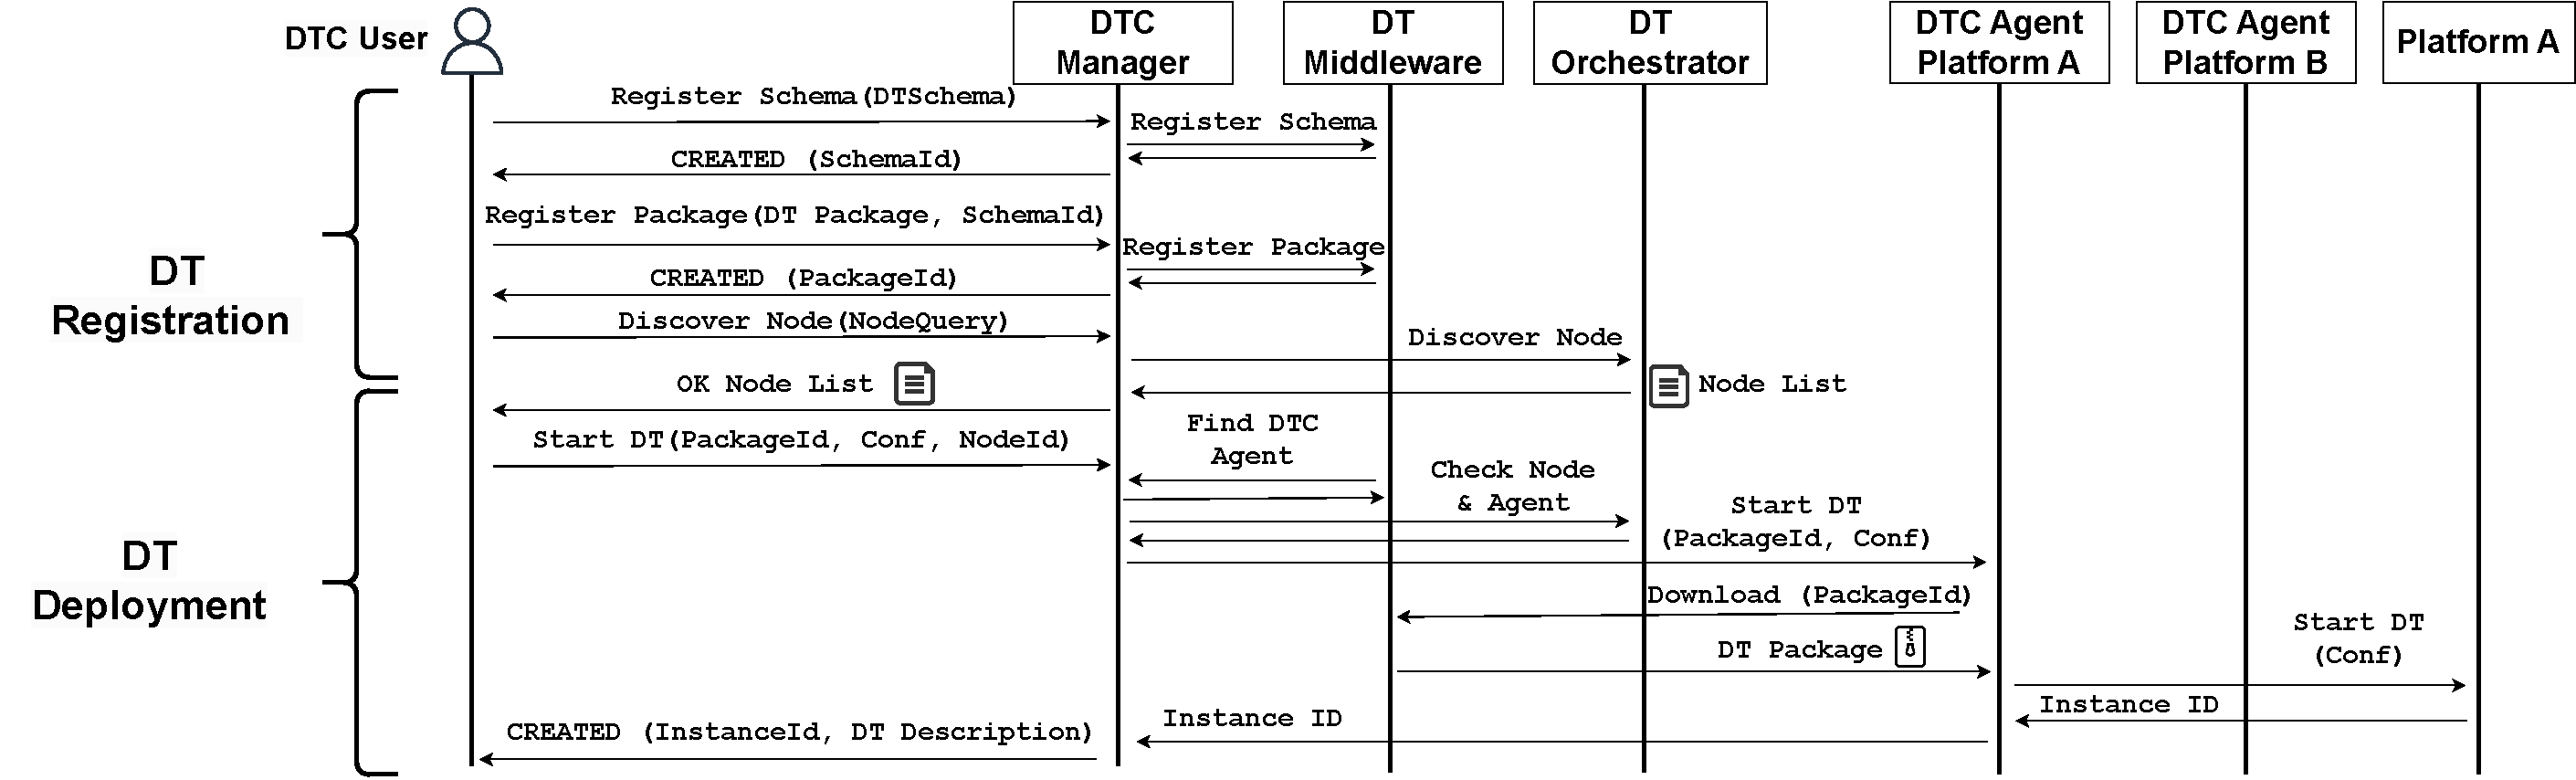
\includegraphics[width=\textwidth]{figures/dtc/sequence_diagram.pdf}
    \caption{The interaction flow example between DTC architectural components to enable DT registration and deployment.}
    \label{fig:dtc-interaction}
\end{figure}

\Cref{fig:dtc-interaction} present an illustrative example depicting a typical interaction scenario among the key components of the DTC architecture.
%
Assuming that the PA has been already registered in the DTC providing the corresponding PAS and PAI descriptions, the figure illustrates the sequence of interactions that occur when a generic user aims to register and deploy a DT for a specific PA.

The initial step to deploy a DT on a target platform involves registering a new DT Schema.
%
All the interactions are facilitated by the DTC Manager, which implements the external-facing API and receives, handles and forwards incoming requests to the appropriate internal component.
%
The request to register a DT Schema is forwarded from the DTC Manager to the DT Middleware. Here, the incoming request is validated, and a new schema is created for the target DT associated with its description, capabilities and fidelity together with the type of physical asset. Subsequently, the DTC manager responds to the user with positive feedback.

The subsequent step entails registering or creating a DT Package linked to the specific schema. The interaction flow follows is similar to the one above, with the DTC Manager receiving the request and the DT Middleware registering the package and associating it with the corresponding SchemaID. 

Moving forward, the registration process for the DTC User involves identifying suitable compute nodes for deploying the target DT. This necessitates a node discovery request initiated by the user, which is forwarded to the DTC Manager.
%
Internally, the DT Orchestrator engages in the discovery process, returning a list of available nodes that match the user's specified criteria, such as the support for package deployment and the support for target hardware requirements (e.g., a GPU for the execution of specific DT's functionalities).
%
The selection of nodes could be automated based on predefined policies. Fort simplicity, in this example, we let the user choose the preferred node from the list of available options.

Upon reviewing the list of available compute nodes matching the target package and schema, the user can proceed by sending a start request to the DTC Manager.
%
This request includes the specific package ID associated with the target schema, along with the starting configuration of the twin which include the identifier of the PAI to which the \ac{DT} will be linked together with the node ID indicating where the DT should be deployed. 
The DTC Manager first verifies compliance of the \ac{DT} package with the platform and the selected PAI, then it checks for the availability of the designated DTC Agent managing the specified node.

Subsequently, it forwards a start request to the target DTC Agent managing the selected platform and node.
%
Here, the DTC Agent checks for the presence of the target DT Package and downloads it if necessary. Once the package is available, the Agent initiates and starts the target DT on the designated platform.
%
Finally, the Agent receives the instance ID of the running DT from the platform and communicates it back to the DTC manager. Subsequently, the DTC manager replies with the instance ID to the user, along with the current description of the running DT instance.

This interaction flow exemplifies the collaborative efforts of the DTC components in facilitating the registration and deployment of DTs, ensuring a seamless experience for users while abstracting the underlying complexities of the infrastructure.
%
By leveraging the descriptions introduced in \Cref{table:dtc_descriptions_requirements}, the DTC effectively manages the lifecycle of DTs, from registration to deployment, while ensuring compatibility with the underlying platforms and compute nodes.

%=======================================================
\section{Proof of Concept Implementation}
%=======================================================


A preliminary analysis, implementation, and experimental evaluation of the core functionalities of the DTC have been conducted using a prototype based on Eclipse Ditto and WLDT as reference platforms.
%
The primary objective of this implementation is to demonstrate the feasibility of the DTC and obtain initial insights by leveraging the microservice capabilities of the White Label Digital Twin (WLDT) library.

The DTC's functional modules (\Cref{fig:dtc-architecture}) are implemented in Python, featuring a \emph{master API} that orchestrates overall behavior and a set of \emph{DTC agents} that manage specific computing nodes and interface with underlying DT platforms such as WLDT and Eclipse Ditto. 
%
These components expose structured RESTful APIs, enabling standardized interaction with the DTC core services. Monitoring and performance tracking across distributed nodes are facilitated through Prometheus, serving as a centralized time-series database, while local agents collect metrics on individual machines.
%
Observability, visualization, and analysis are supported via Grafana dashboards. For the experimental evaluation, the supporting infrastructure—including Virtual Machines (VMs), networking, and container runtimes (Docker and Kubernetes)—was assumed to be preconfigured.


\begin{figure*}[ht!]
    \centering
    \begin{subfigure}{0.49\textwidth}
        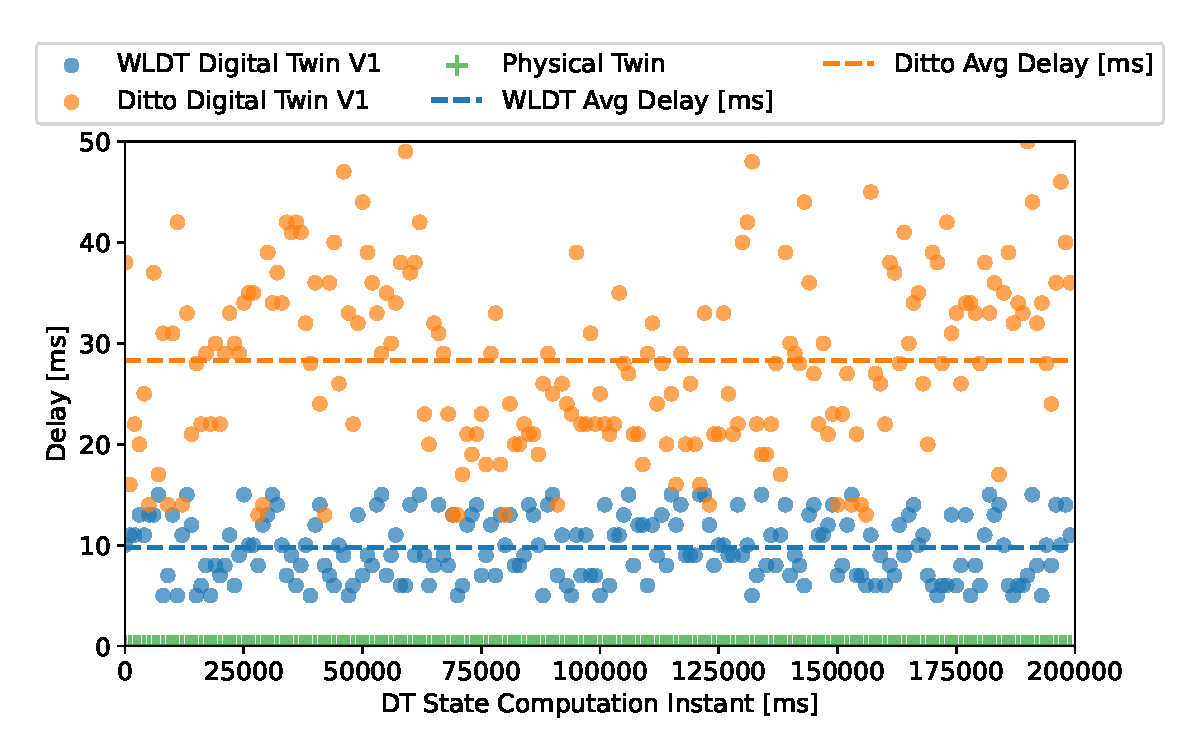
\includegraphics[width=\textwidth]{figures/dtc/wldt_ditto_end_to_end_delay_comparison.pdf}
        \caption{Single DT deployed on both edge and cloud, showing consistent state computation with a small propagation delay between platforms.}
    \end{subfigure}\hfill
    \begin{subfigure}{0.49\textwidth}
        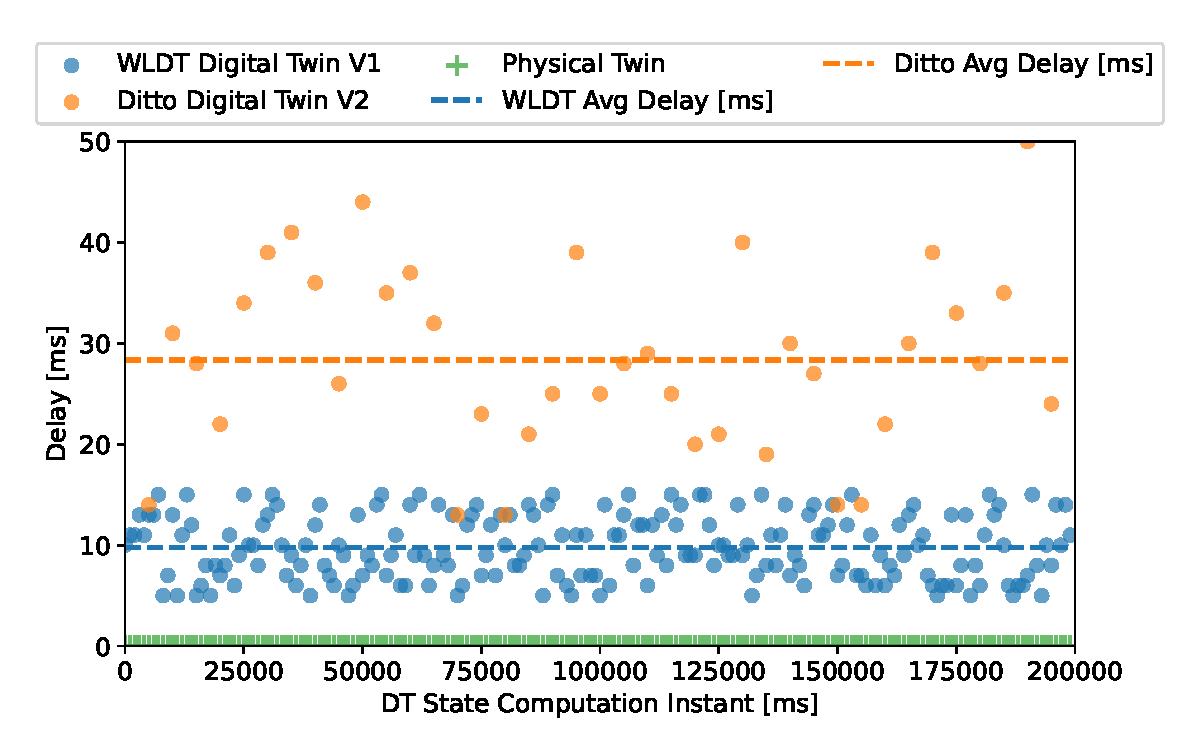
\includegraphics[width=\textwidth]{figures/dtc/wldt_ditto_end_to_end_delay_comparison_2_dts.pdf}
        \caption{Updated cloud DT model with coarser aggregation, illustrating the impact of model versioning and aggregation on state computation relative to the edge DT.}
    \end{subfigure}
    \caption{Comparison of end-to-end DT state computation delays across edge (WLDT) and cloud (Ditto) platforms.}
    \label{fig:exp_single_dt}
\end{figure*}

The \textbf{first experiment} examines the behavior of a single DT deployed across two platforms: WLDT at the edge and Ditto in the cloud. Rather than focusing on communication delays, this experiment aims to demonstrate how the DTC orchestrates state computation and ensures synchronization across multiple DT instances operating on heterogeneous platforms. Two observers, one on the edge and one in the cloud, monitored the propagation and consistency of the DT states.

In the first configuration (Figure \ref{fig:exp_single_dt} left), both DTs run the same model version. The results confirm that the DTC effectively coordinates the two instances, maintaining consistent state computation across edge and cloud, with only minor propagation differences that do not affect overall correctness.

In the second configuration (Figure \ref{fig:exp_single_dt} right), the cloud-based DT is switched to a different, coarser, DT schema (V2) that employs a longer time window for state aggregation (receiving updates from the PA every seconds and computing the state every 5 samples), while the edge DT continues operating with the original high-granularity schema. The DTC seamlessly manages this update, ensuring the cloud DT is correctly deployed and integrated without disrupting the ongoing edge operations. This illustrates the DTC's capability to orchestrate heterogeneous model versions, maintaining consistent, system-wide behavior across distributed DT instances versions and reconcile differences between distributed DT instances.

%%%
\begin{figure}
    \centering
    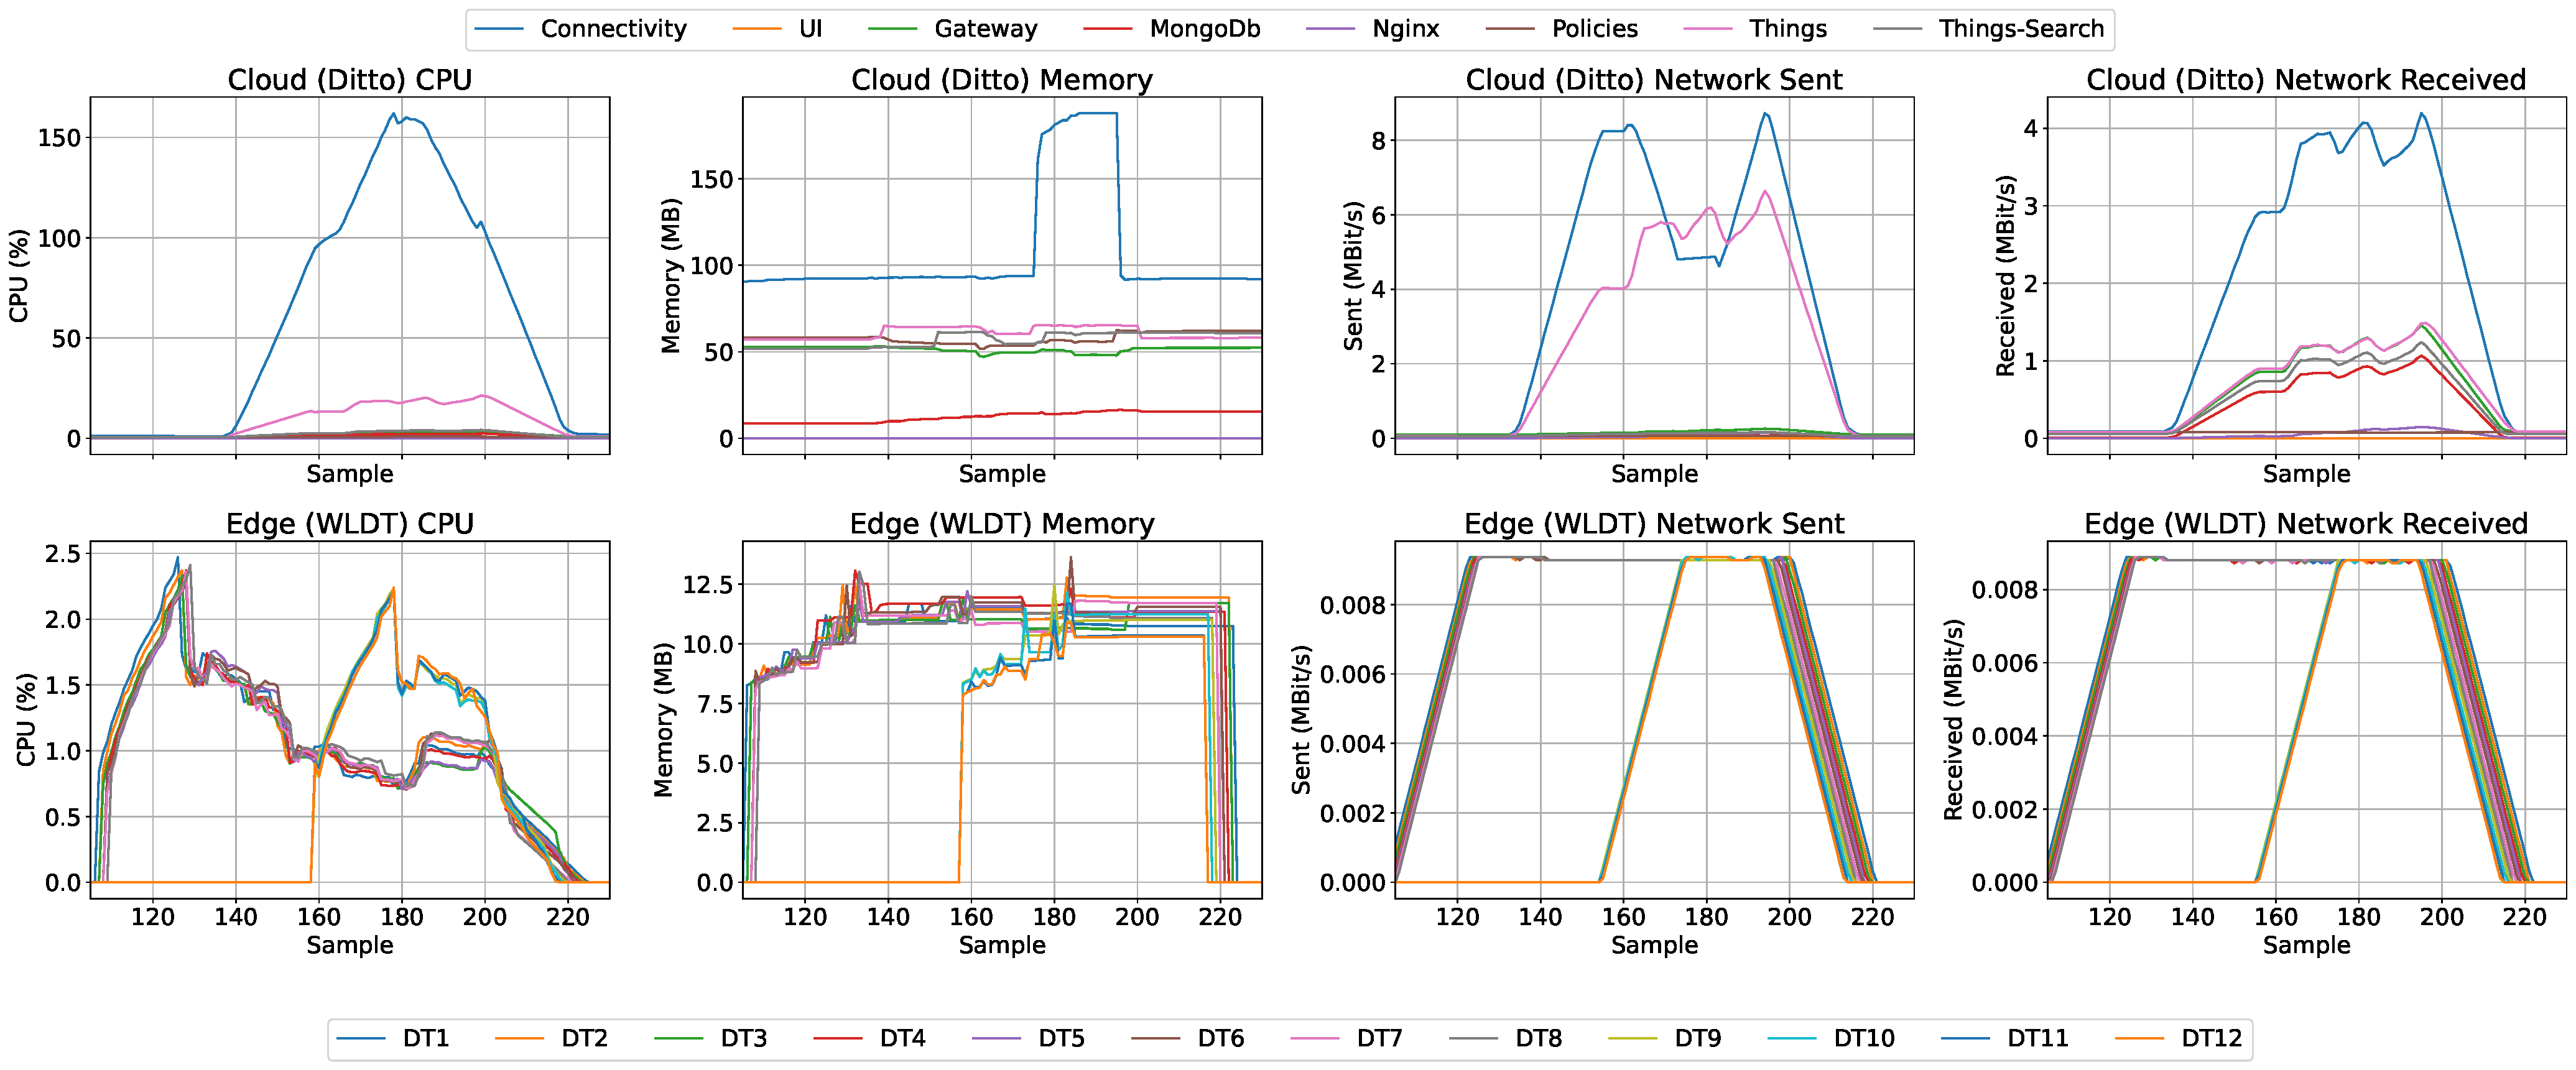
\includegraphics[width=\textwidth]{figures/dtc/edge_cloud_experiment.pdf}
    \caption{Scalability assessment of the DTC prototype in the Microfactory deployment. The figure shows two rows of graphs corresponding to edge (WLDT) and cloud (Ditto) deployments respectively on Edge and Cloud, reporting the evolution of CPU usage, memory consumption, inbound network traffic, and outbound network traffic as the number of active Digital Twin instances increases.}
    \label{fig:dt_resource_usage}
\end{figure}
%%%

The \textbf{second experiment} evaluates the scalability of the DTC prototype in a realistic microfactory deployment (see \Cref{ssec:dte:dt-engineering:scenario} for a description of the microfactory environment).
Performance metrics, including CPU and memory usage as well as network traffic, were monitored during a dual deployment scenario, with Digital Twins instantiated both at the edge (WLDT) and in the cloud (Ditto). The experiment encompasses DTs for individual machines, aggregated DT models for each of the two production lines, and a factory-level DT, totaling twelve distinct DT instances managed by the \ac{DTC}.

Deployment proceeded incrementally along the experimental timeline. Initially, eight DTs were instantiated solely on the edge, followed by the activation of four additional DTs in the cloud, until reaching the full deployment of twelve DTs on both edge and cloud platforms, representing all DT for the microfactory scenario.
%
In this setup, edge DTs exhibit composition behavior compared with the first experiment, while cloud DTs receive their input from edge DTs rather than directly from the physical assets. This configuration allows the DTC to coordinate multiple DT instances across heterogeneous platforms, maintaining synchronization, ensuring consistent communication, and optimizing resource usage as the number of DTs increases.

Measurements captured CPU and memory consumption, as well as inbound and outbound network traffic for each microservice—including core components of Eclipse Ditto and WLDT-based DTs. The results depicted in Figure \ref{fig:dt_resource_usage} illustrate distinct phases of the experiment and highlight the DTC's capability to manage multiple platforms simultaneously. Importantly, the focus is on demonstrating the orchestration and management capacity of the DTC rather than directly comparing the performance of Ditto versus WLDT.

Overall, this proof-of-concept implementation confirms the feasibility and effectiveness of the DTC architecture. The DTC successfully encapsulates the complexity of managing heterogeneous Digital Twin platforms, providing a unified and coherent view of the industrial system across edge and cloud layers, while maintaining scalability, observability, and system performance under growing operational load.

% %=======================================================
% \section{Discussion}
% %=======================================================
\todo{a critical discussion would be nice here but I don't think I'll have time to write it.. }

%=======================================================
\section{Final Remarks}
%=======================================================

This chapter presents the concept of \acl{DTC} as a middleware platform to support the operational management of \ac{DTE} on a compute continuum. 
%
The \ac{DTC} addresses key challenges that emerge when dealing with the deployment and management of systems that involve multiple \acp{DT}, characterized by heterogeneous physical assets, diverse DT platforms, and varying application requirements.

The proposal in this chapter contributes to answering the research question:

\paragraph{\ref{rq:3} How can we support the operational management of DTEs?}

By using structured descriptions that capture the essential characteristics of physical assets, digital twins, and runtime platforms, the DTC enables stakeholders to effectively discover, deploy, and manage DT instances across a distributed infrastructure.
%
The descriptions are designed to be platform and application-agnostic, allowing for seamless integration and interoperability among different DT platforms and use cases.
%
The DTC architecture incorporates key functional components, including a middleware layer and orchestrator, which facilitate the interaction with distributed computing nodes through the abstraction of DTC agents. 
%
This approach supports different stakeholders in their respective roles, offering a coherent holistic view of the DT ecosystem alongside the development-to-deployment lifecycle of its components. 

